
\documentclass{esub2acm}
%\documentclass[11pt]{article}

\usepackage{alltt}
\usepackage{graphicx}
%\usepackage[dvips]{epsfig}
% New mathematical facilities like \mathbb, \big, and \mapsto
%\usepackage{amssymb}
% Defines page size and margins.
%%
%   Preamble
%
%
%   The parameter oddsidemargin (evensidemargin) is one inch 
%   less than the distance from the edge of the paper to the 
%   left margin of the text on right-hand (left-hand) pages. 
%
\setlength{\textwidth}{6.0in}
\setlength{\oddsidemargin}{23pt}
\setlength{\evensidemargin}{23pt}
\setlength{\topmargin}{-0.5in}
\setlength{\textheight}{8.5in}

%   Some abbreviations

\newcommand{\grad}{\nabla}
\newcommand{\bull}{\vrule height 1.8ex width 1.0ex depth 0ex}
\newcommand{\half}{{\textstyle{\frac{1}{2}}}}
\newcommand{\Ref}[1]{\mbox{\rm{(\ref{#1})}}}
\newcommand{\qed}{$ \blacksquare $ \medskip}
\newcommand{\lt}{<}
\newcommand{\gt}{>}
%
%   Enviroments theorem lemma and algorithm are created, and all
%   three are numbered as in theorem.
%
\newtheorem{theorem}{Theorem}
\newtheorem{lemma}[theorem]{Lemma}
\newtheorem{corollary}[theorem]{Corollary}
\newtheorem{algorithm}[theorem]{Algorithm}
\newtheorem{definition}[theorem]{Definition}
\newtheorem{assumption}[theorem]{Assumption}
%
%   The numbering below can be done with the numinsec style
%   provided by SIAM.
%
%   The theorem numbers are defined to be of the form section#.theorem#
%
\renewcommand{\thetheorem}{\thesection.\arabic{theorem}}
%
%   Defines the equation number to be of the form section#.equation#
%
%   \renewcommand{\theequation}{\thesection.\arabic{equation}}
%
%   Defines the figure and table numbers to be of the form 
%   section#.figure# and section#.table#
%
\renewcommand{\thefigure}{\thesection.\arabic{figure}}
\renewcommand{\thetable}{\thesection.\arabic{table}}


% Redefines the size of the section headings.
%\usepackage{../sty/art11mod}
% The float package is described in page 146 of the LaTeX companion.
\usepackage{../sty/float}
% Numbers equations,... consecutively within sections.
%\usepackage{../sty/numinsec}
% The bar package is described in page 283 of the LaTeX companion.
%\usepackage{../sty/bar}
% The url package is intended for email addresses, hypertext links, ...
\usepackage{../sty/url}

%\usepackage[first]{draftcopy}
%\usepackage{subfigure}

% New commands for final copy
\newcommand{\Ref}{\ref}
\newcommand{\half}{\frac{1}{2}}
\newcommand{\lt}{<}
\newcommand{\gt}{>}
\newcommand{\grad}{\nabla}

% New commands
%\newcommand{\R}{\mbox{${\mathbb R}$}}
\newcommand{\R}{\mbox{${\Re}$}}
\newcommand{\Note}{\marginpar[$\Rightarrow$]{$\Leftarrow$}}
% Renewing commands
\renewcommand{\thefootnote}{\fnsymbol{footnote}}
% Algorithm floating environment.
\newfloat{Algorithm}{thp}{loa}[section]

% Calligraphic letter abbreviations.

\newcommand{\cA} {\mbox{$\cal A$}}
\newcommand{\cB} {\mbox{$\cal B$}}
\newcommand{\cD} {\mbox{$\cal D$}}
\newcommand{\cF} {\mbox{$\cal F$}}
\newcommand{\cI} {\mbox{$\cal I$}}

\begin{document}
%\setlength{\baselineskip}{15pt}

%\pagestyle {empty}

%  
\pagestyle{empty}
\hspace{-.65in}
\includegraphics{ArgonneLogo}
\hfill  {\large {\bf ANL/MCS-TM-322 Rev. 3.13}}

\vspace*{2in}
\noindent {\huge{\bf TAO Users Manual}}
\vspace*{8pt}
\hrule
\vspace*{8pt}
\noindent {\Large{\it Revision 3.13}}

\vspace*{1in}
\noindent \\
{\Large {\bf Mathematics and Computer Science Division}}

\vspace*{10pt}


\vspace*{20pt}

%%%%%%%%%%%%%%%%%%%%%%%%%%%%%%%%%%%%%%%%%%%%%%%%%%%%%%%%%%%%%%%%%%%%%%%%%%%%%%%%%%%%

\newpage
\newgeometry{top=0mm, left=0mm, right=0mm, bottom=0mm}
\centerline{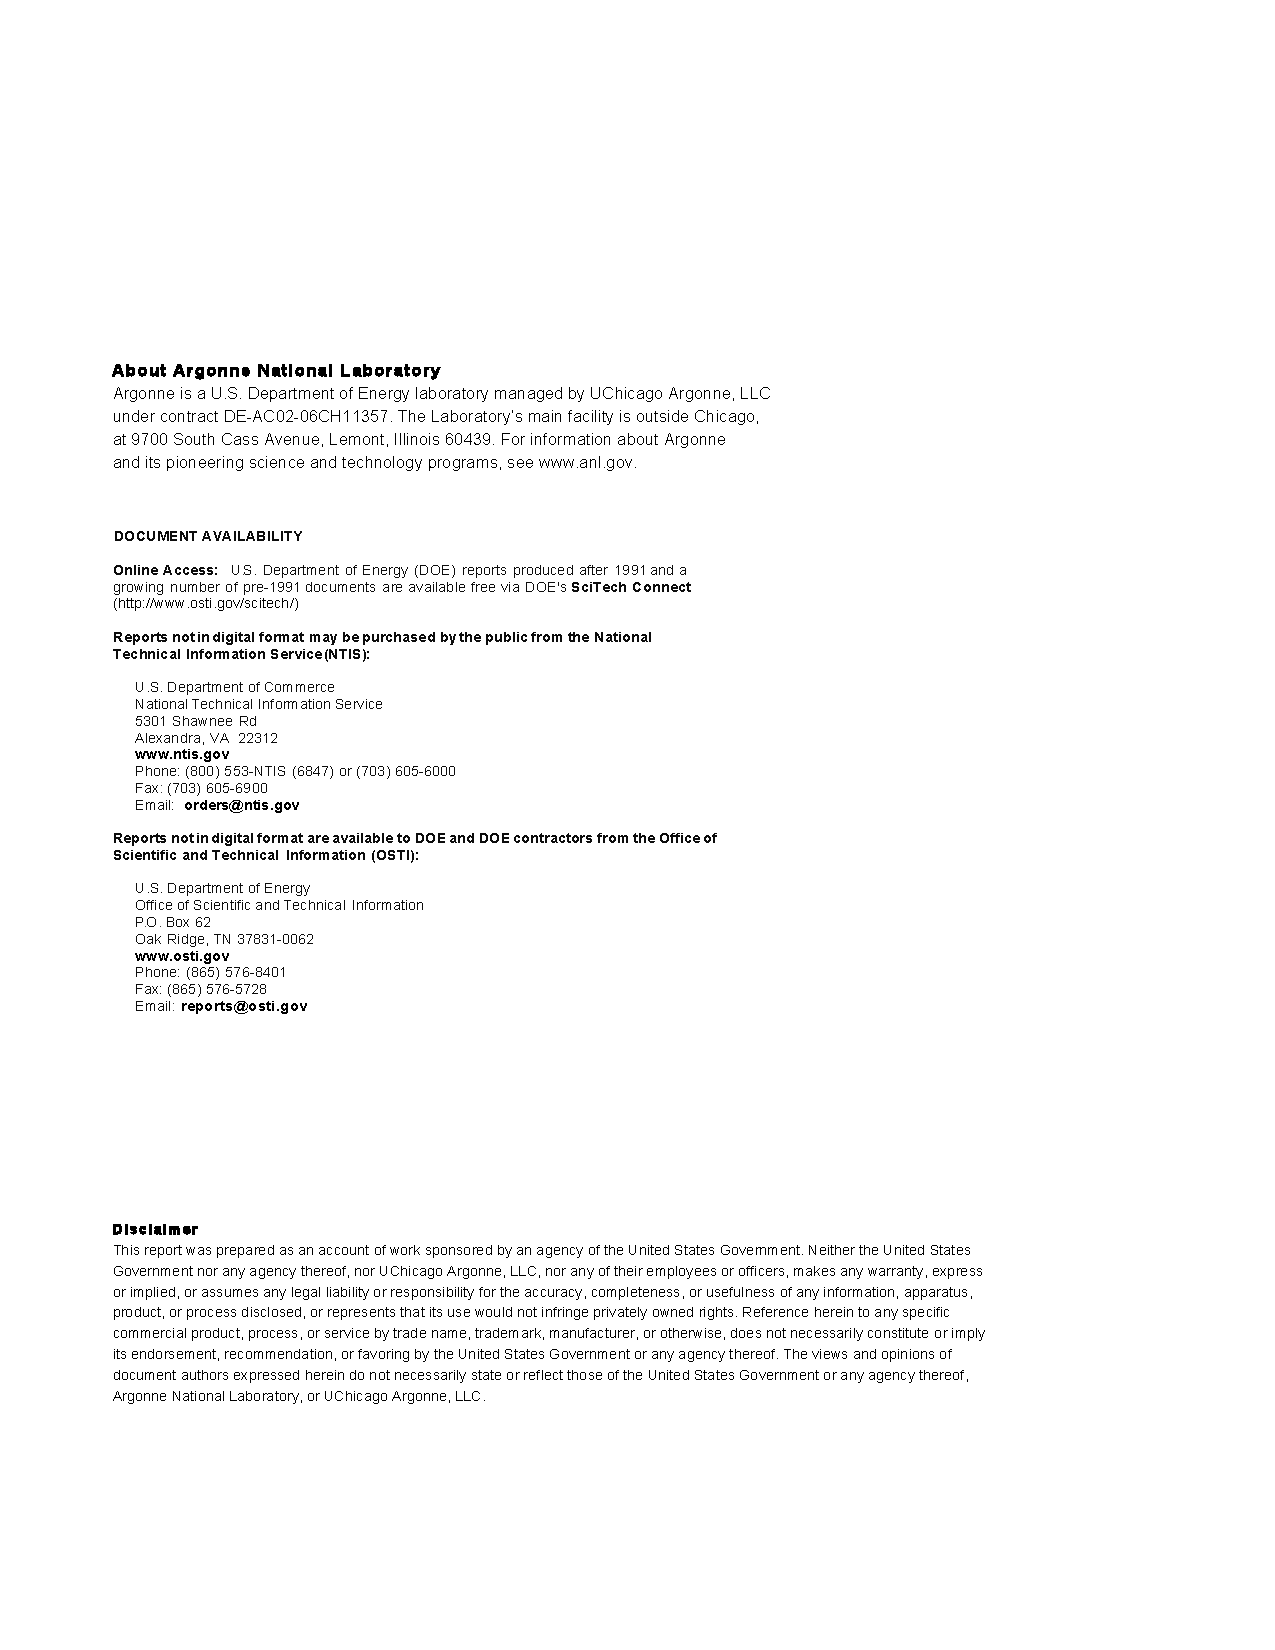
\includegraphics{ArgonneReportTemplatePage2}}
\newpage
\restoregeometry

%%%%%%%%%%%%%%%%%%%%%%%%%%%%%%%%%%%%%%%%%%%%%%%%%%%%%%%%%%%%%%%%%%%%%%%%%%%%%%%%%%%%

\pagestyle{empty}
\hfill {\large {\bf ANL/MCS-TM-322 Rev. 3.13}}

\vspace*{2in}
\noindent {\LARGE{\bf TAO Users Manual}}
\vspace*{8pt}
\hrule
\vspace*{8pt}
\noindent {\Large{\it Revision 3.13}}

\vspace*{0.5in}
\noindent Prepared by \\
{\bf Alp Dener \\ Adam Denchfield \\ Hansol Suh \\ Todd Munson \\ Jason Sarich \\ Stefan Wild \\ Steven Benson \\ Lois Curfman McInnes}\\

\vspace*{30pt}
\noindent March 2020

\vspace*{20pt}
\noindent This work was supported by the Office of Advanced Scientific Computing Research, \\
Office of Science, U.S. Department of Energy, under Contract DE-AC02-06CH11357.

%  \newpage
%  \mbox{}
%  \newpage

%\pagestyle{plain}


\title{A Case Study in the Performance and Scalability of
Optimization Algorithms\footnotemark}

\author{Steven J. Benson
\and
Lois Curfman McInnes
\and
Jorge J. Mor\'e \\
Mathematics and Computer Science Division \\
Argonne National Laboratory
}

\begin{abstract}
We analyze the performance and scalabilty of algorithms for the
solution of large optimization problems on 
high-performance parallel architectures.
Our case study uses the GPCG (gradient projection, conjugate gradient) algorithm
for solving bound-constrained convex quadratic problems.
Our implementation of the GPCG algorithm within the Toolkit for 
Advanced Optimization (TAO) is available
for a wide range of high-performance architectures
and has been tested on problems with over 2.5 million variables.
We analyze the performance as a function of the number of variables, 
the number of
free variables, and the preconditioner.
In addition, we discuss how the software
design facilitates algorithmic comparisons.
\end{abstract}

%  \noindent
%  {\bf Key words.} 
%  large-scale optimization,
%  high-performance architectures,
%  conjugate gradients, 
%  gradient projection,
%  quadratic programming., 

\category{G.4.m} {Mathematical Software} {Parallel and vector implementations}
\category{D.2.13} {Reusable Software} {Reusable libraries}
\category{G.1.6}{Optimization}{Quadratic Programming Methods}
\terms{Bound constrained optimization, Parallel Efficiency}
\keywords{}
\begin{bottomstuff}
This work was supported by the Mathematical, Information, and
Computational Sciences Division subprogram of the Office of Advanced
Scientific Computing, U.S. Department of Energy, under Contract
W-31-109-Eng-38.
\begin{authinfo}
\end{authinfo}
\permission
\end{bottomstuff}
\markboth{S.J. Benson, L. McInnes, J.J. Mor\'e}
     {A Case Study in the Performance and Scalability of
Optimization Algorithms}
\maketitle


\section{Introduction}
In this paper, we describe how variable metric methods can be applied
in a subspace defined by a set of linear equalities.
Then we descibe an algorithm that applies these methods to solve
large nonlinear optimization problems with simple bounds
on the variables.  We write this problem as
\begin{equation} \label{def_bqp}
\min \{ f(x) : l \leq x \leq u \} ,
\end{equation}
where $f : \R^n \mapsto \R $ is a nonlinear function whose gradient
$\nabla f$ is available, the vectors $l$ and $u$ are fixed, and the 
inequalities are taken componentwise.
Since the algorithm does not require second derivatives, the
method can be applied when the Hessian is not available or not
practical to compute.


The method in this paper is similar to the ones in Byrd, Lu, Nocedal,
and Zhu\cite{Byrd:1995:LMA} in that we create a quadratic model function using
gradient information in such a way that the storage required in linear in $n$.
The main difference, however, is that while they use gradients 
to construct the model function and then minimize the model over a 
sequence of subspaces,
we use projected gradients
to generate the model function and compute a search direction in
the full space of variables.

\section{Bound Constrained Optimization Problem}\label{qp}

A classical result shows that the bound-constrained 
optimization problem (\ref{def_bqp}) has a  unique solution
on the feasible region
\begin{equation} \label{def_bounds}
\Omega = \{ x \in \R^n: l \leq x \leq u \}
\end{equation}
when the function $f : \R^n \mapsto R $ is strictly convex.
This result holds for unbounded $\Omega$, and we thus
allow the components of $l$ and $u$ to be infinite.
Solutions to problem \Ref{def_bqp} satisfy the Kuhn-Tucker conditions
\[ \begin{array}{lllll}
\partial_if(x) & = & 0 & \mbox{ if } & x_i \in (l_i, u_i) \\
\partial_if(x) & \geq & 0 & \mbox{ if } & x_i = l_i \\
\partial_if(x) & \leq & 0 & \mbox{ if } & x_i = u_i ,\\
\end{array}
\]
where $\partial_if(x)$ is the partial derivative of $f$ with
respect to the $i$th variable.

The projection operator 
\begin{equation} \label{projection-tangent}
 \left[ \tc d \right] _i = \left\{
\begin{array}{lll}
d_i & \mbox{ if } & x_i \in (l_i, u_i) \\
\min \{ d_i,0 \} & \mbox{ if } & x_i = l_i \\
\max \{ d_i,0 \} & \mbox{ if } & x_i = u_i
\end{array}
\right.
\end{equation}
can be helpful in our analysis
because $x^*$ is a solution of (\ref{def_bqp}) if and only if
the projected gradient $\tcc \nabla f(x^*) =0$.
Given a tolerance $\tau$, an
approximate solutions to the bound constrained problem (\ref{def_bqp}) 
is any vector $x \in \Omega$ such
that
\begin{equation} 
\label{bqp_approximate_sol}
\| \tc \nabla f(x) \| \leq \tau . % \| \grad f(x_0) \| .
\end{equation}
Note that (\ref{bqp_approximate_sol}) holds whenever
$x$ is sufficiently close to $x^*$ and in the face of $\Omega $ that
contains $x^*$.  

The concept of a face is standard in convex analysis;
for the convex set (\ref{def_bounds}), the face of $\Omega$ that contains
$x$ is
\[ 
\Bigl \{ y \in \Omega: y_i = x_i \mbox{ if } x_i \in \{ l_i, u_i \} \Bigr \}. 
\]
Thus, the face of the feasible set that contains $x$ can
be described in terms of the set of active constraints
\[
\cA (x) = \{ i: x_i = l_i \mbox{ or } x_i = u_i \}. 
\]
Variables with indices in ${\cal A}(x)$ are the active variables,
and those with indices outside  ${\cal A}(x)$ are the free variables.
Similarly, the binding variables are those with indices in
\[ 
\cB (x) = \{ i:x_i=l_i \mbox{ and } \partial_if(x) \geq 0,
\mbox{ or } x_i=u_i \mbox{ and } \partial_if(x) \leq 0 \}. 
\]
The Kuhn-Tucker conditions show that 
$ \cB (x) = \cA (x) $ at a solution.
%, so that if all the active
% variables are not binding, then $x$ is not on the face
% that contains the solution.  True?


\section{Reduced Space and Subspace Variable Metric Methods}\label{alg}

A standard transformation of variables can reduce the problem
\begin{equation} \label{def_red}
\min \{ f(x) : A x = b \},
\end{equation}
where $ A \in \R^{(n-p) \times n}$, $b \in \R^{n-p}$
into an unconstrained optimization problem in $p$ variables.
Given a point $x_0$ such that $A x_0 = b$ and a matrix $Z \in \R^{n \times p}$ 
whose columns are orthonormal ($Z^T Z = I$) and span the nullspace of $A$ ($A Z = 0$), 
all points $x$ satisfying
$A x = b$ can be written as $x = x_0 + Z \overline{x}$ for some $\overline{x} \in \R^{p}$.
The vector $\overline{x}$ lies in a {\it reduced space} of $\R^n$
and the vector $Z \overline{x}$ lies in a {\it subspace} of  $\R^n$.
An objective function 
$\overline{f} : \R^p \mapsto \R $ 
in the reduced space can be the written as
\[ \overline{f}(\overline{x}) = f( \hat x +  Z \overline{x}) \]
The gradient vector and Hessian matrix of this function can be written as
\[ \begin{array}{rl}
\nabla \overline{f}(\overline{x}) &= Z^T \nabla f( \hat x +  Z \overline{x}) \\
\nabla^2 \overline{f}(\overline{x}) &= Z^T \nabla f( \hat x +  Z \overline{x}) Z \\
\end{array} \]

There are many algorithms for unconstrained optimization that
have proven effective in theory and practice, and the BFGS algorithm,
in particular, has been a popular choice.
The BFGS method approximates the Hessian with the 
correction pairs
$\{ s_i, y_i\} $ 
such that
\begin{equation}\label{defsy}
s_i = x_{i+1} - x_{i} \hspace{0.5in} \mbox{ and }  \hspace{0.5in} 
y_i= \nabla f(x_{i+1}) - \nabla f(x_{i}).
\end{equation}
Given an initial matrix $H_k$ that approximates the inverse Hessian matrix,
a new approximation $H_{k+1}$ is defined by the recursive formula
\begin{equation}\label{defbfgs}
H_{k+1} = V_{k}^T H_{k} V_{k} + \rho_k s_{k} s_k^T 
\end{equation}
where 
\begin{equation}\label{defrho}
\rho_k = \frac{1}{\langle y_k, s_k \rangle} \hspace{0.5in} \hbox{ and } \hspace{0.5in} V_k = I - \rho_k y_k s_k^T. 
\end{equation}
This matrix can easily be seen to be positive definite if
${H}_{k}$ is positive definite and  $\langle y_k, s_k \rangle > 0$.
The matrix $H_{k+1}$ minimizes $\| H - H_k \|_{W}$
subject to constaints that $H=H^T$ and $H y_k = s_k$.
The matrix norm $\| A \|_{W} = \| W^{1/2} A  W^{1/2} \|_{F}$
where $W$ is any matrix satisfying the secant equation
$W {y}_k = {s}_k$ and $\| A \|_F$ is the Frobenius norm.
We will refer the matrix $H_k$ defined by 
(\ref{defsy}), (\ref{defbfgs}) and (\ref{defrho})
as the {\bf full BFGS matrix}.
 
%The solution to the model function
%(\ref{q-model}) is given by $-H_k \nabla f(x_k)$.
With the updated matrix $H_k$, the BFGS method defines
$x_{k+1} = x_k - \alpha_k H_k \nabla f(x_k)$
for some positive step length $\alpha_k$.
Any line search that enforces the Wolfe conditions will generate
a step length that produces
a new point and gradient such that $\rho_{k+1}> 0$.
A more complete discussion of the method and its properties 
can be found in \cite{NW99}.


In a affine subspace $A x = b$, the BFGS step direction can be generalized.

\begin{definition}\label{D1}
Let $Z \in \R^{n \times p} $ be a matrix with orthonormal columns.
Given a symmetric positive definite matrix 
$\overline{H}_k \in \R^{p \times p}$ 
and a correction pair
$\{ \overline{s}_k , \overline{y}_k \} $ such that
$\overline{s}_k = Z^T x_{k+1} - Z^T x_k $,
$\overline{y}_k = Z^T \nabla f(x_{k+1}) - Z^T \nabla f(x_k)  $, 
and
$\overline{\rho}_{i} = 1 / \langle \overline{y}_i, \overline{s}_i \rangle > 0$,
define the
{\bf reduced BFGS matrix} with respect to Z, $\overline{H}_{k+1}$, to be
\begin{equation}\label{defbfgsbar}
\overline{H}_{k+1} = \overline{V}_{k}^T \overline{H}_{k} \overline{V}_{k} + 
\overline{\rho}_k \overline{s}_{k} \overline{s}_k^T 
\end{equation}
where 
\begin{equation}\label{defrhobar}
\overline{\rho}_k = \frac{1}{\langle \overline{y}_k,\overline{s}_k \rangle} 
\hspace{0.5in} \hbox{ and } \hspace{0.5in} 
\overline{V}_k =\overline{I} - \overline{\rho}_k \overline{y}_k \overline{s}_k^T. 
\end{equation}
\end{definition}
The matrix $\overline{H}_{k+1}$ minimizes
$ \| \overline{H} - \overline{H}_k \|_W $ subject to the constraints that
$\overline{H}_{k+1}$ is symmetric and
$\overline{s}_k = \overline{H} \overline{y}_k$.   The
matrix norm used here is analagous the one used is the unconstrained
BFGS method except that that matrices must satisfy the reduced secant
equation $\overline{s}_k = W \overline{y}_k$.
When there are no
linear constraints, $p=n$, $Z=I$, and $\overline{H}_{k+1} = {H}_{k+1}.$

\comment{The matrix norm $\| A \|_{W} = \| W^{1/2} A  W^{1/2} \|_{F}$
where $W$ is any matrix satisfying the secant equation
$W \overline{y}_k = \overline{s}_k$ and $\| A \|_F$ is the Frobenius norm. 
This matrix can easily be seen to be positive definite if
$\overline{H}_{k}$ is positive definite and  $\overline{s}_k^T \overline{y}_k > 0$.
A more complete discussion of the method and its properties 
can be found in \ref{NW99}.
}

\begin{example}
Consider the following bound constrained problem
\begin{equation} \label{def_ex}
\min \{ f(\chi_1,\chi_2,\chi_3) =  \chi_1^2 - \chi_1 \chi_2  + 0.75 \chi_2^2 + 0.5 \chi_3^2 + 4 \chi_1 - 4 \chi_2 - 2 \chi_3 : \chi_3 \geq 0 \} ,
\end{equation}
which has a unique minimum at $(0, 8/3, 2)$.  The optimal face is 
\[ \{ (\chi_1,\chi_2,\chi_3) : \chi_1 = 0; \}, \]
so fix $\chi_1=0$ and consider the unconstrained problem in variables $\chi_2$ and $\chi_3$.
Here $Z \in \R^{3 \times 2}$ and its columns are the second and third columns of the
identity matrix.

The gradient of $f$ is defined by
\[
\nabla f = [ 2 \chi_1 - \chi_2 + 4, -\chi_1 + 1.5 \chi_2 - 4 , \chi_3  - 2  ]^T
\]
and 
\[
\nabla f(0,0,0) = [ 4, -4, -2]^T, 
\hspace{1.0in}
\nabla f(0,2,1) = [ 2, -1 , -1]^T
\]

Start the algorithm at the origin, step in the direction of the gradient to
where $\overline{x}_1 = [ 2, 1]^T$.  This step sets
$\overline{y}_0 = [3, 1]^T$ and $\overline{s}_0 = [2, 1]^T$.
If $\overline{H}_0 = \overline{I}$, then
\[
\overline{H}_1 =
\left[
\begin{array}{cc}
33/49  & -1/49   \\
-1/49  &  52/49  \\
\end{array}
\right],
\comment{ 
\hspace{1in}
\overline{H}_1^{-1}=
\left[ \begin{array}{cc}
52/35  & 1/35   \\
1/35  &  33/35  \\
\end{array} \right]
}
\]
the secant equation holds, and
\[
\overline{H}_1 Z^T \nabla f(0,2,1) = \overline{H}_1 [ -1 , -1 ]^T = [ -32/49 , -51/49 ]^T.
\]
\end{example}

The reduced BFGS matrix is not, however, the same as the
matrix $Z^T H_k Z$.  More importantly, the step direction
generated by the reduced BFGS matrix is not the same as the
step directions $\left[ Z^T H_k Z \right]  \left[ Z^T \nabla f(x_k) \right]$
or  $\left[ Z^T H_k \nabla f(x_k) \right]$

\begin{example}
Consider the bound constrained problem in Example 1.
Let $H_0 = I$ and $H_1$ be the full BFGS matrix.  
Start at the origin at step in the direction of the
projected gradient to  $x_1 = [0, 2, 1]^T$.
The correction pairs
\[
y_0 = [-2, 3, 1]^T;  \hspace{1in} s_0 = [ 0, 2, 1]^T
\]
produce
\[
H_1 =
\left[     
\begin{array}{ccc}
1     & 4/7   &  2/7 \\
4/7  &  1    &  1/7 \\
2/7  &  1/7  &  8/7 \\
\end{array}
\right],
\comment{
H_1^{-1} =
\left[ \begin{array}{ccc}
11/7   & -6/7   & -2/7 \\
-6/7  &  52/35   & 1/35 \\
-2/7  & 1/35  &  33/35 \\
\end{array} \right].
}
\]
The matrix
$Z^T H_1 Z 
\comment{ = \left[     
\begin{array}{cc}
1    &  1/7 \\
1/7  &  8/7 \\
\end{array}
\right]
}
$
clearly does not equal $\overline{H}_1$.
The step directions $ Z^T {H}_{1} \nabla f(x_1) $  and
$Z^T {H}_{1} Z Z^T \nabla f(x_1)$
in the reduced space do not equal the step direction generated from the reduced BFGS matrix.
That is,
\[ Z^T H_1 \nabla f(0,2,1) = Z^T [ 8/7, 0, -5/7]^T = [ 0, -5/7]^T \neq \overline{H}_1 Z^T \nabla f(0,2,1)\]
and
\[Z^T H_1 Z Z^T \nabla f(0,2,1) = [ -8/7, -9/7]^T \neq \overline{H}_1 Z^T \nabla f(0,2,1).\]
Furthurmore, the reduced secant equation does not hold, 
\[Z^T H_1 Z \overline{y}_0 = [ 22/7 , 11/7]^T   \neq \overline{s}_0. \]
\end{example}

Any step direction, $\overline{ \Delta x}$, in the reduced space can be
mapped into a step direction in the full space, $ \Delta x$, 
by $ \Delta x = Z \overline{ \Delta x}$.  In Example 1, the full
step direction $Z  \overline{H}_1 Z^T \nabla f(x_1) = [0, -32/49, -51/49 ]^T$.
This direction is different from the full space directions
generated in Example 2.

In some instances, it may be inconvenient to work explicitly
in the reduced space.
In optimization problems with linear inequalities, 
for instance, the subspace may change from one iteration to the next.   
The cost of creating reduced space data structures, mapping data into
them, and computing the reduced BFGS matrix at each iteration could
be prohibitably expensive.
%and Example 2 shows that the reduced matrix $ Z^T H Z $ is not sufficie
In these contexts, it
is convenient and more efficient 
to update the BFGS matrix in the full space and then
reduce these matrices in the appropriate space.
Even better,
we would like to develop methods that build a matrix in the
full space and generate directions in a subspace that coincide with
the directions generated by the reduced space BFGS method.


Specifically, these methods should generated matrices ${H}_{k}$ such that
\begin{equation}\label{P1}
Z^T {H}_{k} d =  \overline{H}_{k} Z^T d,  \forall d \in \R^n.
\end{equation}
If (\ref{P1}) is true, the step direction, 
$Z \overline{H}_k Z^T \nabla f(x_k)$,
generated in the reduced space and mapped to the full space 
equals the direction,
$Z Z^T H_k \nabla f(x_k)$, generated in the full space and projected
into the subspace.

\begin{example}
Multiples of the identity matrices $cI$ and $c\overline{I}$ satisfy (\ref{P1}).
for all real  $c$.
\end{example}

\begin{example}
Some implementations of the BFGS algorithm for unconstrained optimization
select $H_0$ after the first iterate using a 
correction pair $\{ s, y \}$.
In particular, suppose
$\overline{H}_0 = \langle \overline{s} , \overline{y} \rangle /
\langle  \overline{y},  \overline{y} \rangle \overline{I} $
and
$H_0 = \langle s , y \rangle / \langle y , y \rangle I$.
$\overline{H}_0$ and $H_0$
satisfy (\ref{P1}) if and only if $y = Z Z^T y$.  
\end{example}

\begin{theorem} \label{T11}
Assume a matrix $Z$ such that $Z^T Z = I$ and matrices $H_k \in \R^{n \times n}$
and $ \overline{H}_{k}^{p \times p}$ that satisfy
\[ Z^T {H}_{k} d =  \overline{H}_{k} Z^T d,  \hspace{0.5in} \forall d \in \R^n. \]
Furthermore, assume correction pairs
${s}_k , {y}_k  \in \R^n$ such that $\langle s_k, y_k \rangle > 0$ and
$\langle Z^T s_k, Z^T y_k \rangle > 0$, define
$\overline{s}_k = Z^Ts_k$, $\overline{y}_k = Z^Ty_k$.  
If 
${H}_{k+1}$ is the matrix 
defined by  (\ref{defbfgs}) and (\ref{defrho}), and
$\overline{H}_{k+1}$ is the reduced BFGS matrix 
defined by (\ref{defbfgsbar}) and (\ref{defrhobar}),
then
\[ Z^T {H}_{k+1} d =  \overline{H}_{k+1} Z^T d ,  \hspace{0.5in}  \forall d \in \R^n.\]
if and only if
$s_k = Z \overline{s}_k $ and $y_k = Z \overline{y}_k$.
\end{theorem}

\proof{
First assume that $s_k = Z \overline{s}_k $ and $y_k = Z \overline{y}_k$.  This
implies that
$\overline{\rho}_{k} = \rho_k$ and
\[
\begin{array}{ll}
 Z^T {H}_{k+1} d  &=  Z^T (I - \rho_k s_k y_k^T) H_k (I - \rho_k y_k s_k^T) d + \rho_k Z^T s_k s_k^T d \\
&=  Z^T (I - \overline{\rho}_k Z \overline{s}_k  \overline{y}_k^T Z^T) H_k 
        (I - \overline{\rho}_k Z \overline{y}_k  \overline{s}_k^T Z^T) d + +  \overline{\rho}_k Z^T Z \overline{s}_k \overline{s}_k Z^T d \\
&=  (I - \overline{\rho}_k  Z^T Z \overline{s}_k  \overline{y}_k^T ) Z^T H_k 
    (I - \overline{\rho}_k  Z \overline{y}_k  \overline{s}_k^T Z^T) d + 
\overline{\rho}_k \overline{s}_k \overline{s}_k^T Z^T d \\
&=  (I - \overline{\rho}_k  Z^T Z \overline{s}_k  \overline{y}_k^T ) \overline{H}_{k} Z^T
    (I - \overline{\rho}_k  Z \overline{y}_k  \overline{s}_k^T Z^T) d + 
\overline{\rho}_k \overline{s}_k \overline{s}_k^T Z^T d \\
&=  (I - \overline{\rho}_k  Z^T Z \overline{s}_k  \overline{y}_k^T ) \overline{H}_{k}
    (I - \overline{\rho}_k  Z^T Z \overline{y}_k  \overline{s}_k^T ) Z^T d + 
\overline{\rho}_k \overline{s}_k \overline{s}_k^T Z^T d \\
&=  (I - \overline{\rho}_k  \overline{s}_k  \overline{y}_k^T ) \overline{H}_{k}
    (I - \overline{\rho}_k  \overline{y}_k  \overline{s}_k^T ) Z^T d + 
\overline{\rho}_k \overline{s}_k \overline{s}_k^T Z^T d \\
& = \overline{H}_{k+1} Z^T d
\end{array}
\]

Conversely, assume that
\[ Z^T {H}_{k+1} d =  \overline{H}_{k+1} Z^T d ,  \forall d \in \R^n.\]
Then 
\begin{equation} \label{pp1}
 \begin{array}{ll}
Z^T {H}_{k+1} ( s - Z \overline{s} )  &= \overline{H}_{k+1} Z^T  ( s - Z \overline{s} ) \\
&= \overline{H}_{k+1} (Z^T s - Z^T Z \overline{s} ) \\
&= \overline{H}_{k+1} ( \overline{s} - \overline{s}) \\
&= 0.
\end{array} \end{equation}
By similar arguments,
\begin{equation} \label{pp2} Z^T {H}_{k} ( s_k - Z \overline{s}_k ) = 0, \end{equation}
\begin{equation} \label{pp3} Z^T {H}_{k+1} ( y_k - Z \overline{y}_k ) = 0, \end{equation}
and
\begin{equation} \label{pp4} Z^T {H}_{k} ( y_k - Z \overline{y}_k ) = 0. \end{equation}
For any vector $e \in \R^n$,
\begin{equation} \label{pp5}
\begin{array}{ll}
Z^T {H}_{k+1} e
&= Z^T (I - \rho_k s_k y_k^T) H_k (I - \rho_k y_k s_k^T) e + \rho_k Z^T s_k s_k^T e \\
&= Z^T H_k e - \rho_k Z^T s_k y_k^T H_k e - Z^T H_k \rho_k y_k s_k^T e + \rho_k^2  Z^T s_k y_k^T H_k y_k s_k^T e + \rho_k Z^T s_k s_k^T e \\
&= Z^T H_k e  - \rho_k \overline{s}_k y_k^T H_k e - \rho_k  \overline{H}_k Z^T y_k s_k^T e + \rho_k^2 \overline{s}_k y_k^T H_k y_k s_k^T e + \rho_k \overline{s}_k s_k^T e \\
&= Z^T H_k e + ( -\rho_k y_k^T H_k e + \rho_k^2 y_k^T H_k y_k s_k^T e  +\rho_k s_k^T e ) \overline{s}_k -
(  \rho_k s_k^T e )  \overline{H}_k \overline{y}_k
\end{array}
\end{equation}
If $e = s - Z \overline{s}$, then by (\ref{pp1}),(\ref{pp2}), and (\ref{pp5}), 
\[ ( -\rho_k y_k^T H_k e + \rho_k^2 y_k^T H_k y_k s_k^T e  +\rho_k s_k^T e ) \overline{s}_k -
(  \rho_k s_k^T e )  \overline{H}_k \overline{y}_k = 0 . \]
Since $ \overline{s}_k$ and $\overline{H}_k \overline{y}_k$
may be linearly independent and $\rho_k > 0$, the coefficients
$ - y_k^T H_k e + \rho_k y_k^T H_k y_k s_k^T e  + s_k^T e = 0 $
and $ s_k^T e = 0$.
The equations
\[
s_k^T e = s_k^T (s_k - Z  \overline{s}_k)
= s_k^T s_k - s^T Z \overline{s}_k
= s_k^T s_k - \overline{s}_k^T \overline{s} \\
\]
and
\[ \| e \|^2  = s_k^Ts_k - \overline{s}_k^T \overline{s}_k - \overline{s}_k^T \overline{s}_k +  \overline{s}_k^T \overline{s}_k 
= s_k^Ts_k - \overline{s}_k^T \overline{s}_k,\]
imply that
$s_k = Z \overline{s}_k$.

To prove that $y_k = Z \overline{y}_k$, let  $e = y_k - Z \overline{y}_k$.  
By (\ref{pp3}), (\ref{pp4}), (\ref{pp5}), and the same argument as above,
$s_k^Te = 0$ and $y_k^T H_k e = 0$.

Since
\[ \begin{array}{ll}
y_k^T H_k e &= y_k^T H_k (y_k - Z \overline{y}) \\
&= (y_k - Z \overline{y}_k)^T H_k (y_k - Z \overline{y}_k) + ( Z \overline{y}_k)^T H_k (y_k - Z \overline{y}_k) \\
&= (y_k - Z \overline{y}_k)^T H_k (y_k - Z \overline{y}_k) + \overline{y}_k^T Z^T  H_k (y_k - Z \overline{y}_k) \\
&= (y_k - Z \overline{y}_k)^T H_k (y_k - Z \overline{y}_k) \\
\end{array} \]
and $H_k$ is positive definite, the equation 
$y_k^T H_k e = 0$ implies that $y_k - Z \overline{y}_k$.
}

\begin{corollary} \label{T22}
Given the assumptions of Theorem \ref{T11}, define 
$ \overline{s}_k = Z^T \left( x_{k+1} -  x_{k} \right) $
and $ \overline{y}_k = Z^T \nabla f(x_{k+1}) -  Z^T \nabla f(x_{k}) $.
If $H_k$ and $\overline{H}_k$ are also defined in Theorem \ref{T11},
then $ Z^T {H}_{k+1} d =  \overline{H}_{k+1} Z^T d $ if and only
if $y_k = Z Z^T \nabla f(x_{k+1}) - Z Z^T \nabla f(x_{k})$
and $s_k = Z Z^T \left( x_{k+1} - x_{k} \right) $.
\end{corollary}

This corollary states that $x_{k+1} - x_k$ must
lie in the subspace and that $y_k$ is the difference
of gradients that are projected into the subspace.

\begin{corollary} \label{T33}
If $y_k = Z Z^T \nabla f(x_{k+1}) - Z Z^T \nabla f(x_{k})$,
$s_k = Z Z^T \left( x_{k+1} - x_{k} \right)$, and
$ Z^T {H}_{k} d =  \overline{H}_{k} Z^T d $
for all $d \in \R^n$, then the step direction
$Z^T H_{k+1} \nabla f(x_{k+1}) $ generated in the full space equals \
the direction  $\overline{H}_{k+1} Z^T \nabla f(x_{k+1}) $ generated in the
reduced space, and 
$Z Z^T H_{k+1} \nabla f(x_{k+1}) = Z \overline{H}_{k+1} Z^T \nabla f(x_{k+1})$.
\end{corollary}

Other reduced space methods use the reduced Hessian matrix
$Z^T \nabla^2 f(x) Z$ and its inverse.
It is very tempting generate a step direction in the
reduced space using the reduced matrix $Z^T H Z$.  However,
the matrix $H$ approximates the inverse Hessian matrix, not
the Hessian matrix, and the property
\[ \left[ Z^T B Z \right]^{-1} = Z^T B^{-1} Z \]
is generally not true for $B$ equal to an exact Hessian or 
approximations of it.
Therefore the matrix this matrix  $Z^T H Z$ 
is not same as the matrix generated using this
matrix may not generate the reduced BFGS step direction.
If the matrix $B$ and its inverse $H$ are 
constructed according to Theorem \ref{T11}, then
this equality holds, the step generated in the reduced space
will be the true BFGS step direction, and the full matrix $H$ can be
used to generate BFGS step directions.

\begin{example}
Consider the bound constrained problem in Example 1.
Start at the origin at step in the direction of the
projected gradient to  $x_1= [ 0, 2, 1 ]$.
Define 
$s_i = x_{i+1} - x_{i}$ and
$y_i= \tc \nabla f(x_{i+1})  - \tck \nabla f(x_{i})$ so that
\[ y_0 = [ 0,3,1];  \hspace{1in} s_0 = [0,2,1]. \]
Then 
\[
H_1 =
\left[     
\begin{array}{ccc}
1 &  0 &  0 \\
0 &  33/49  & -1/49   \\
0 &  -1/49  &  52/49  \\
\end{array}
\right], 
\]
In the reduced space,  the step direction
$Z^T H_1 \nabla f(0,2,1) = Z [-32/49, -51/49 ]^T$ equals the
step direction produced by the reduced BFGS matrix, and
in the full space $Z Z^T H_1 \nabla f(x) = Z \overline{H}_1 Z^T \nabla f(x)$.
The reduced secant equation
$Z^T H_1 Z \overline{y} = \overline{s}^T$
also holds.
\end{example}

In this example, the conditions
$y = Z \overline{y}$ , 
and $s = Z \overline{s}$ are true in addition to
the standard conditions that
$\overline{y} = Z^T y$ and $\overline{s} = Z^T s$, 


\section{BLMVM}

Like the unconstrained BFGS method, BLMVM creates 
a convex quadratic model function
\begin{equation}\label{q-model}
m_k(d) = f(x_k) + \nabla f(x_k)^T {d} +
\half {d}^T B_k {d}.
\end{equation}
The matrix $B_k$ will be updated
at each iteration using correction pairs $s_k$ and $y_k$.
Letting $H_k = B_k^{-1}$,
the minimizer $d_k$ of this of this quadratic
can be written explicitly as
$d_k = - H_k \nabla f(x_k)$ and used as a step direction in
the algorithm

Unlike the unconstrained BFGS method, however, BLMVM defines the
correction pairs
\begin{equation}\label{correction}
s_k = x_{k+1} - x_{k}, \hspace{1in} 
y_k= \tc \nabla f(x_{k+1})  -\tc \nabla f(x_k)
\end{equation}
to update $H_k$. This choice of correction pairs is 
motivated two observations.  The first observation
is that just as the norm of the gradient will converge to zero as $x_k$ 
converges to an unconstrained minimum, 
the norm of the projected gradient should converge to zero as
$x_k$ converges to a bound constrained minimum.
The second observation pertains the theory provided in the previous section.
This choice of $y_i$ is like updating the BFGS matrix in the space
of nonbinding variables. For points sufficiently near the
solution, the set of binding variables correctly identifies
the face with the optimimal solution.

Since the inverse Hessian approximation is usually dense, 
the cost of storing $H_k$ and manipulating it is prohibitive for
large problems.  To reduce these costs, the L-BFGS method stores a 
limited number of correction pairs $\{ s_i, y_i\}$,
$i = k-m, \ldots, k-1$. 
Once the number of correction vectors exceeds the number of vectors available
to store them, a new correction pair is added by removing the oldest one.
Given an initial inverse Hessian approximation $H_k^0$, 
the L-BFGS algorithm defines
\begin{equation}\label{lbfgs}
\begin{array}{ll} 
H_k = &\left( V_{k-1}^T \ldots  V_{k-m}^T \right) H_k^0 \left( V_{k-m} \ldots  V_{k-1} \right) \hspace{0.05in} + \\
& \rho_{k-m} \left( V_{k-1}^T \ldots  V_{k-m+1}^T \right) s_{k-m} s_{k-m}^T  \left( V_{k-m+1} \ldots  V_{k-1} \right) \hspace{0.05in} + \\
& \ldots \hspace{0.05in} + \\
& \rho_{k-2} \left( V_{k-1}^T \right) s_{k-2} s_{k-2}^T  \left( V_{k-1} \right) \hspace{0.05in} + \\
& \rho_{k-1} s_{k-1} s_{k-1}^T.
\end{array}
\end{equation}
%This matrix can easily be seen to be positive definite if $H_k^0$ is 
%positive definite and $\rho_i >0$ for all $i$.  
This representation of the matrix provides
an efficient solution to the quadratic problem (\ref{q-model}).
Given any $m$ correction pairs $\{ s_i, y_i\}$ such that 
$\{ s_{k-m}, y_{k-m}\}$ is the least recent pair and
$\{ s_{k-1}, y_{k-1}\}$ is the most recent pair,
the operation action $\hat d := H_k v$
can be computed using the pseudo code\cite{NW99}:

\begin{Algorithm} [ht]
\noindent{\bf L-BFGS two-loop recursion}:
\begin{list}{}
{
\setlength{\parsep}{0pt}
\setlength{\itemsep}{0pt}
\setlength{\topsep}{0pt}
}
\item $\hat d \leftarrow  v$
\item for $i=k-1, \ldots, k-m $

\begin{itemize}
\item $\beta_i \leftarrow { \rho_i}{\langle \hat d, s_i \rangle } ;$
\item $\hat d \leftarrow \hat d - \beta_i y_i;$
\end{itemize}

\item $\hat d \leftarrow H_k^0 \hat d ;$

\item for $i= k-m, \ldots, k-1$
\begin{itemize}
\item $\hat d \leftarrow \hat d + \left( \beta_i - { \rho_i }{ \langle \hat d , y_i \rangle 
} \right) s_i $
\end{itemize}

\end{list}
\end{Algorithm}


to generate a step direction 
\[\hat d = - H_k \nabla f(x_k) .\]

The matrix $H_k^0$ can change from one iteration to the next; 
BLMVM used the limited memory BFGS matrix and selects
$H_k^0 = \langle s_k , y_k \rangle / \langle y_k , y_k \rangle I$.

The computational cost of computing $s_i$, $y_i$, $\rho_i$, $\|y_i\|$, and
this pseudo code is $(8m+9)n$ flops, which
is dominated by the
cost of evaluating $f(x_k)$ and $\nabla f(x_k)$ in many applications.


\comment{This choice of correction pairs allows us to generate a good 
step direction in the space of nonbinding variables 
without explicitly working in this subspace of $\Omega$.
}

Our algorithm uses a projected line search to
enforce the bounds of the variables.
We select a step length $\alpha_k$ and
define $x_{k+1} = P [x_k + \alpha_k {d_k} ]$.
The operator $P$ is a projection
onto $\Omega$ and can be computed in $n$ operations by
\[ 
P[x] = \mbox{ mid} (l,u,x), 
\]
where $\mbox{ mid} (l,u,x)$ is the vector whose $i${th} component
is the median of the set $\{ l_i, u_i, x_i \} $.

Since there may not exist a step length that satisfies the Wolfe conditions,
we apply a simple backtracking method to select a step size such that
\begin{equation}  \label{gplsstop}
 f(x_{k+1}) \leq f(x_k) + \mu
\langle \nabla f(x_k), x_{k+1} - x_k \rangle
\end{equation}
for some $\mu \in (0, 1/2 )$.
The step size is computed by setting $ \alpha_k $
to the first member of the sequence
$ \gamma_0 ( \half ) ^ j $ for $ j = 0, 1, \ldots $ such that
$ x_{j+1} $ satisfies the sufficient decrease condition \Ref{gplsstop}.
The choice of $\gamma_0$ is the infimum of $1.0$ and all
$\gamma > 0$ such that
$P [x_k + \gamma {d_k} ] = P [x_k + \hat \gamma {d_k}] $  
for all $\hat \gamma \geq  \gamma$.
This line search allows the set of active and binding variables to
change by more than one variable at each iteration.  This choice
of line search also means that we that we do not have to
explicitly project the direction $H \nabla f(x)$.
More sophisticated projected searches are possible,
but this simple search has proved to be sufficient in all cases tried.

Condition (\ref{gplsstop}) is true for sufficiently small $alpha_k$ if 
$\langle - \tcc H_k \nabla f(x_k) , \nabla f(x) \rangle \leq 0$.
When there are finite bounds on the variables, the set of
binding variables may
change significantly in the early iterates.
Although $-H_k \nabla f(x_k)$ will always be a
descent direction since $H_k$ is positive definite,
the direction $-\tcc H_k \nabla f(x_k)$
may not be a descent direction.
In the event that 
$\langle \tcc H_k \nabla f(x_k) , \nabla f(x) \rangle \leq 0$,
we let $d=-\tcc \nabla f(x_k)$.  
In  practice, we have found that projected gradients rarely
need to be used as a step direction.

The algorithm can be summarized as follows:

\begin{Algorithm}
\noindent{\bf Algorithm BLMVM}: 
Choose $ x_0 \in \Omega $. Let $d = - \tcc \nabla f(x_0)$.   
For $ k = 0, \ldots, $
\begin{list}{}
{
\setlength{\parsep}{0pt}
\setlength{\itemsep}{0pt}
\setlength{\topsep}{0pt}
}
\item[1.]
Compute $\alpha_k$ using a projected line search and let
$x_{k+1} = P [x_k + \alpha_k {d_k}]$.

\item[2.]
Compute $\nabla f(x_{k+1})$ and  its projection $\tcc \nabla f(x_{k+1})$.

\item[3.]
If $\| \tcc \nabla f(x_{k+1}) \| < \epsilon $, stop.

\item[4.] 
Compute $y_{k}$ and $s_{k}$ according to (\ref{correction}).  
If $y_{k}^Ts_{k} > 0$, update $H_{k}$.

\item[5.] 
Compute $H_{k+1} \nabla f(x_{k+1}) $ using the L-BFGS two-loop recursion.

\item[6.]
If $\langle -\tcc (H_{k+1} \nabla f(x_{k+1})),\nabla f(x_{k+1})\rangle > 0$,
let $d=- H_{k+1} \nabla f(x_{k+1})$;
otherwise let $d=-\nabla  f(x_{k+1})$.

\end{list}
\end{Algorithm}


For points sufficiently close to the solution, not only does 
$\overline{y}_k = Z^T y_k$  and $\overline{s}_k = Z^T s_k$ , but
$y_k = Z \overline{y}_k$ and $s_k = Z \overline{s}_k$.
If the $m$ correction pairs stored by the algorithm possess
this property, the algorithm will generate the same direction
in the reduced space as applying the L-BFGS algorithm in 
the reduced space.


\begin{theorem} \label{L1}
Let $Z \in \R^{n \times p}$ be a matrix whose columns are
the columns of the identity matrix corresponing to the
nonbinding variables.  Furthermore, 
et $\overline{H}_k$ be the reduced L-BFGS matrix on the set
of nonbinding variables at $x_k$ and let $H_k$ be the
quasi Newton matrix generated by (\ref{correction}), (\ref{defrho}),
and (\ref{defbfgs}).
If
\begin{enumerate}
\item[(i)]   $x_{k-m}, \ldots, x_{k}$ lie on the same face, and
\item[(ii)]  $\cB (x_{k-m}) = \ldots = \cB (x_{k}) =\cB (x^*) $, 
\end{enumerate}
then 
\begin{equation} \label{TT44}
\tcc ( H_k \nabla f(x_k) ) = Z \overline{H}_k Z^T \nabla f(x_k). 
\end{equation}
\end{theorem}

\proof{
The definition of $\tcc$ and $Z$ is such that 
$\tcc  \nabla f(x_k) = Z Z^T  \nabla f(x_k)$.  As in Example 4,
The matrix $H_k^0$ satisfies (\ref{TT44}).
By the first condition,
$s_k = Z Z^T (x_{k+1} - x_{k})$ for $i=k-m, \ldots, k-1$.
By the second condition, $y_k = Z Z^T \nabla f(x_{k+1}) - Z Z^T \nabla f (x_{k})$  for $i=k-m, \ldots, k-1$.
Therefore, by Theorem \ref{T11} and Corollary \ref{T33}, the statment holds.
\comment{Since the binding variables are a subset of the active variables,
condition (i) implies that
$[x_{k-m}]_i = \ldots = [x_k]_i$ for all $i \in \cB (x)$
and $[s_{k-m}]_i = \ldots = [s_{k-1}]_i = 0$ for all $i \in \cB (x)$.
Condition (ii) implies that
$\left[ \tcc f(x_{k-m}) \right]_i = \ldots = 
\left[ \tcc f(x_k) \right]_i = 0$
and $[y_{k-m}]_i = \ldots =[y_{k-1}]_i = 0$ for all $i \in \cB (x)$.

$[ P[x_k - c \nabla f(x_k)] ]_i = [x_k]_i $ 
Since the vectors $y_k$ and $s_k$ equal zero in all of the
for all of the binding  variables,

Therefore the scalings are the same and the conclusion holds.
}
}

Note:  For what problems will this condition hold close to the solution.?

This theorem obviously applies when 
the lower bounds equal $-\infty$ and the upper bounds
equal $\infty$ because no variable is ever binding.
The  theorem also applies when $x_{k-m}, \ldots, x_{k}$ lie 
sufficiently close to the solution $x^*$ and on the same
face as the solution.

Even when the iterates are on a face other than the optimal
one, the step directions are very good.  The reason is that
the gradient with respect to variables that are likely to
equal one of the bounds will have little effect upon the 
step direction.

%%% Local Variables: 
%%% mode: latex
%%% TeX-master: "blmvm"
%%% End: 

\section{Bound-Constrained Quadratic Optimization Problem}

\label{qp}

We assume that the quadratic $q : \R^n \mapsto \R $ is strictly convex
on the feasible region
\begin{equation} \label{def_bounds}
\Omega = \{ x \in \R^n: l \leq x \leq u \} .
\end{equation}
This assumption guarantees that the bound-constrained 
quadratic optimization problem (\ref{def_bqp}) has a unique solution
in  $\Omega$.
Also note that since $q$ is strictly convex, we can define
\begin{equation} \label{def-quadratic}
q(x) = \half \langle x , {A} x \rangle + \langle b , x \rangle + c,
\end{equation}
where $A \in \R^{n \times n}$ is symmetric and
positive definite, $ b \in \R^n$, and $c \in \R$.

We allow the feasible set \Ref{def_bounds} to be unbounded,
and thus the components of $l$ or $u$ can be infinite.
We also allow variables to be fixed by setting $ l_i = u_i $.
If $ l_i < u_i $, then  solutions to problem \Ref{def_bqp} 
satisfy the Kuhn-Tucker conditions
\[ \begin{array}{lllll}
\partial_iq(x) & = & 0 & \mbox{ if } & x_i \in (l_i, u_i) \\
\partial_iq(x) & \geq & 0 & \mbox{ if } & x_i = l_i \\
\partial_iq(x) & \leq & 0 & \mbox{ if } & x_i = u_i , \\
\end{array}
\]
where $\partial_iq(x)$ is the partial derivative of $q$ with
respect to the $i$th variable.
Approximate solutions can be defined in terms of the projected
gradient, defined by
\begin{equation} \label{proj-gradient}
 \left[ \nabla _{\Omega} q(x) \right] _i = \left\{
\begin{array}{lll}
\partial_i q(x) & \mbox{ if } & x_i \in (l_i, u_i) \\
\min \{ \partial_i q(x),0 \} & \mbox{ if } & x_i = l_i \\
\max \{ \partial_i q(x),0 \} & \mbox{ if } & x_i = u_i .
\end{array}
\right.
\end{equation}
This definition of a projected gradient is appropriate 
% for the bound constrained problem (\ref{def_bqp}) 
because $x^*$ is a solution of (\ref{def_bqp}) if and only if
$\nabla_{\Omega} q(x^*)=0$.

Given $x_0 \in \Omega$, and a tolerance $\tau$, an
approximate solution to the bound constrained problem (\ref{def_bqp}) 
is any vector $x \in \Omega$ such
that
\begin{equation} 
\label{bqp_approximate_sol}
\| \nabla_{\Omega} q(x) \| \leq \tau . % \| \grad q(x_0) \| .
\end{equation}
Note that (\ref{bqp_approximate_sol}) holds whenever
$x$ is sufficiently close to $x^*$ and in the face of $\Omega $ that
contains $x^*$.  The concept of a face is standard in convex analysis;
for the convex set (\ref{def_bounds}), the face of $\Omega$ that contains
$x$ is
\[ 
\Bigl \{ v \in \Omega: v_i = x_i \mbox{ if } x_i \in \{ l_i, u_i \} \Bigr \}. 
\]
Thus, the face of the feasible set that contains $x$ can
be described in terms of the set of active constraints
\[ 
{\cal A}(x) = \{ i: x_i = l_i \mbox{ or } x_i = u_i \}. 
\]
Variables with indices in ${\cal A}(x)$ are the active variables,
and those with indices outside  ${\cal A}(x)$ are the free variables.
Similarly, the binding variables are those with indices in
\[ 
{\cal B}(x) = \{ i:x_i=l_i \mbox{ and } \partial_iq(x) \geq 0,
\mbox{ or } x_i=u_i \mbox{ and } \partial_iq(x) \leq 0 \}. 
\]
The Kuhn-Tucker conditions show that 
$ \cB (x) = \cA (x) $ at a solution, so that if all the active
variables are not binding, then $x$ is not on the face
that contains the solution.


\section{The GPCG Algorithm}

\label{alg}

The GPCG algorithm uses a gradient projection method
to identify a face of the feasible region $ \Omega $
that contains the solution, and the conjugate gradient
method to search the face.
This section provides an outline of the algorithm and notes any
differences between our implementation and the implementation
of Mor\'e and Toraldo \cite{more-toraldo}.

Given $y_0=x_k$,
the gradient projection method generates a sequence of vectors $\{y_j\}$
in the feasible region $\Omega$ such that
\begin{equation} \label{next-y}
y_{j+1} = P [ y_j - \alpha_j \nabla q(y_j) ],  
\end{equation}
where $P$ is the projection
onto (\ref{def_bounds}), and
the step size $\alpha_j$ is chosen such that
\begin{equation}  \label{gplsstop}
 q(y_{j+1}) \leq q(y_j) + \mu
\langle \nabla q(y_j), P [ y_j - \alpha_j \nabla q(y_j) ] - y_j \rangle
\end{equation}
for some $\mu \in (0, 1/2 )$.
The projection $P$ can be computed in $n$ operations by
\[ 
P[x] = \mbox{ mid} (l,u,x), 
\]
where $\mbox{ mid} (l,u,x)$ is the vector whose $i${th} component
is the median of the set $\{ l_i, u_i, x_i \} $.
The step size is computed by a
projected search \cite{more-toraldo} by setting $ \alpha_j $
to the first member of the sequence
$ \alpha_0 ( \half ) ^ j $ for $ j = 0, 1, \ldots $ such that
$ y_{j+1} $ satisfies the sufficient decrease condition \Ref{gplsstop}.
In our implementation, we use
\begin{equation} \label{bqpls}
\alpha_{0}= \arg \min 
\left \{ 
q \left (y_j - \alpha  \nabla_{\Omega} q(y_j) \right ):
\alpha > 0 
\right \} .
\end{equation}
Computation of $ \alpha_0 $ is straightforward, since 
the mapping 
$ \alpha \mapsto 
q \left (y_j - \alpha  \nabla_{\Omega} q(y_j) \right ) $ is
a quadratic.

We generate gradient projection
iterates until sufficient progress is not made or
the active set settles down.
Thus, we generate iterates until either
\begin{equation} 
\label{pgstop1}
 {\cal A}(y_j) = {\cal A}(y_{j-1})
\end{equation}
or the condition
\begin{equation} 
\label{pgstop2}
 q(y_{j-1}) - q(y_j) \leq \eta_1 \max \{q(y_{l-1}) - q(y_l) : 1 \leq l < j \},
\end{equation}
holds for some tolerance $ \eta_1 $ in $ (0,1) $.
If either test is satisfied, we proceed to the
conjugate gradient part of the algorithm.

The first test (\ref{pgstop1}) measures when the
active set settles down. For nondegenerate problems, 
(\ref{pgstop1}) holds in a neighborhood of the solution.
The gradient
projection could be followed until the optimal face is found, but
experience has shown that a large number of iterates may be required.
The second test (\ref{pgstop2}) measures when
the gradient projection method is not making sufficient progress.

Given an iterate $x_k$ and the active set  ${\cal A}(x_k)$,
the conjugate gradient method computes an approximate
minimizer to the subproblem
\begin{equation} \label{cg}
\min \{ q(x_k + d): d_i = 0, i \in {\cal A}(x_k) \}.
\end{equation}
This problem is unconstrained in the free variables.  Note that
if $x_k$ lies in the same face as the solution and $d_k$ solves
(\ref{cg}), then $x_k + d_k$ is the solution of (\ref{def_bqp}).

The conjugate gradient algorithm for solving
\Ref {cg} is implemented by expressing
this subproblem in terms of an equivalent subproblem in the
free variables.
Let $ i_1, \ldots, i_{m_k} $
be the indices of the free variables, and let
the matrix $Z_k$ be the matrix in $\R^{n \times m_k} $ whose
$j$th column is the $i_j$th column of the identity matrix in
$\R^{n \times n}$. With this notation we see that
subproblem \Ref{cg} is equivalent to the
unconstrained subproblem
\begin{equation}
\min \{ q _ k ( w ) : w \in \R ^ { m_k } \}  ,
\label{cg2}
\end{equation}
where
\[
q_k(w) \equiv q ( x _ k + Z _ k  w ) - q ( x_k ) =
\half \langle w , {A_k} w \rangle + \langle r_k , w \rangle  .
\]
The matrix $ A_k $ and the vector $ r_k $ are, respectively, the
reduced Hessian matrix of $q$ and reduced gradient of $q$ at $x_k$
with respect to the free variables.
If $A$ is the Hessian matrix of the quadratic $q$, then
\[
A_k = Z_k^T A Z_k , \qquad r_k = Z_k^T \nabla q(x_k)  .
\]
Also note that $A_k$ is the matrix obtained from
$A$ by taking those rows and columns whose indices correspond
to free variables;
similarly, $r_k$ is obtained from $\nabla q(x_k)$ by
taking the components whose indices correspond to free variables.

Given a starting point $ w_0 \in \R^{m_k} $, the conjugate gradient algorithm
generates a sequence of iterates $ w _ 0 , w_1 , \ldots $
that terminates at a solution
of subproblem \Ref {cg2} in at most $m_k$ iterations.
We use the conjugate gradient algorithm 
until it generates $ w _ j $ such that
\begin{equation}
q_k ( w_{j-1} ) - q_k ( w _ {j} ) \le \eta_2 \max \{
q_k ( w_{l-1} ) - q_k ( w _ {l} ) : 1 \le l \lt j \}
\label{cgstop1}
\end{equation}
for some tolerance $ \eta_2 > 0 $. 
The approximate 
solution of \Ref {cg} is then
$ d _ k = Z_k w _ {j_k} $, where $j_k$ is the first index $j$
that satisfies \Ref {cgstop1}.

The termination test \Ref{cgstop1} is not standard.
Iterative solvers usually terminate when
\[
\| r_j + A_j w_j \| \le \eta_2 \|r_j\| 
\]
for some tolerance $\eta_2 \in (0,1) $.
This test suffers from the erratic behavior
of the residual $ \| r_j + A_j w_j \| $.
On the other hand, the termination test \Ref{cgstop1}
depends on  whether the conjugate gradient method
is making sufficient progress.

Given the direction $ d_k $, we use a projected
search \cite{more-toraldo} to define 
$ x_{k+1} = P [ x_k + \alpha_k d_k] $, where
$ \alpha_k $ is the first element in
the sequence $ ( \half ) ^ k $ for $ k = 0, 1, \ldots $ such that
\begin{equation}  \label{cglsstop2}
 q( x_{k+1} ) \le  q(x_k) + \mu
\langle \nabla q(x_k), x_{k+1} - x_k \rangle .
\end{equation}
More sophisticated projected searches are possible \cite{more-toraldo}
,
but this simple search has proved to be sufficient in all cases tried.
If
\begin{equation}
\label{cgstop3}
\cB ( x_{k+1} ) = \cA ( x_{k+1} ) ,
\end{equation}
then we find a more
accurate solution to subproblem \Ref{cg2} by reducing $ \eta_2 $
and continuing with the conjugate gradient method.
Otherwise, we terminate this iteration.

\begin{Algorithm}
\noindent{\bf Algorithm GPCG}
\begin{list}{}
{
\setlength{\parsep}{0pt}
\setlength{\itemsep}{0pt}
\setlength{\topsep}{0pt}
}
\item[]
Choose $ x_0 \in \Omega $.
\item[]
For $ k = 0, \ldots, $
\begin{list}{$\bullet$}
{
% \setlength{\parsep}{0pt}
% \setlength{\itemsep}{0pt}
% \setlength{\topsep}{0pt}
}
\item[]
Set $y_0 = x_k$, and generate gradient projection iterates
$y_1, \ldots, y_{j_k}$, where $j_k$ is the first index to satisfy
(\ref{pgstop1}) or (\ref{pgstop2}). 
Set $x_k= y_{j_k}$.

\item[]
Set $ w_0 = 0 $, and
generate conjugate gradient iterates $ w_1 , \ldots, w_{j_k} $
for the reduced system (\ref{cg}).
Set $ d _ k = Z_k w _ {j_k} $, where $j_k$ is the first index
that satisfies \Ref {cgstop1}.
\item[]
Use a projected search to generate $ x_{k+1} $.
If \Ref{cgstop3} holds, reduce $\eta_2$, and
continue with the conjugate gradient method.
\end{list}
\end{list}
\end{Algorithm}

Our outline of algorithm GPCG does not include the termination test.
An advantage of the termination test \Ref{bqp_approximate_sol} is 
that this test is satisfied \cite{JVB92}
in a finite number of iterations.
On nondegenerate problems GPCG terminates \cite{more-toraldo}
at the solution in a finite number of iterations.

Algorithm GPCG is suitable for large problems.
As opposed to some other active set methods,
each iteration is capable of
adding or removing multiple constraints from the active set.
Moreover, as we shall see, GPCG tends to require few iterations
for convergence.
Another advantage of the GPCG algorithm is that convergence
can be achieved while requiring only approximate solutions
to the linear systems.




\section{Software Design} \label{design}

The TAO design philosophy uses object-oriented techniques of data and
state encapsulation, abstract classes, and limited inheritance to
create a flexible optimization toolkit.  This section provides a short
introduction to our design philosophy by describing the objects needed
to create GPCG and the importance of this design.   

At the algorithmic level, we use objects such as matrices, vectors, 
index sets, and linear solvers.  
Our current implementation leverages the parallel computing
and linear algebra infrastructure offered by 
PETSc~\cite{petsc,PETSc-user-ref},
which employs MPI \cite{using-mpi} for all interprocessor communication.
In this context, a vector ({\texttt Vec}) is an abstraction of an
array of values that represent a discrete field, and a matrix
({\texttt Mat}) represents a discrete linear operator that maps
between vector spaces.  An index set ({\texttt IS}) is a
generalization of a set of integer indices, which can be used for
selecting, gathering, and scattering subsets of vector and matrix
elements.  TAO also interfaces to the preconditioned conjugate gradient 
method and other linear solvers within
PETSc.  Through the \texttt{SLES} component of PETSc, users can define an iterative method,
its preconditioner, and the solution tolerance.
Because each of these objects has several underlying 
representations, TAO has easy access to a variety of parallel vector
and sparse matrix implementations as well as preconditioners and
Krylov subspace methods.
% Functional support for the objects includes the
% creation, duplication, and destruction of the objects.

With sufficiently flexible 
abstract interfaces, TAO can support a variety of implementations of 
data structures and algorithms.  These abstractions allow us
to more easily experiment with a range of algorithmic and data
structure options for realistic problems, such as within this case
study.  Such capabilities are critical for making high-performance
optimization software adaptable to the continual evolution of parallel
and distributed architectures and the research community's discovery
of new algorithms that exploit their features.

The interface to TAO uses only these objects, and a
context variable called \texttt{TAO\_SOLVER}, which encapsulates
information about the solution process, including the algorithm,
convergence tolerances, options, and parameters.  All of the
computations and communications related to a particular solution
process are managed in the solver context variable.  This context
must be created through the  \texttt{TaoCreate} routine, which
specifies the optimization method (denoted by
\texttt{TaoMethod}) and the MPI communicator, which specifies the
processes involved in the optimization computations.

To define the problem, the routine 
\texttt{TaoSetQuadraticFunction} in Figure \ref{tao_interface}
sets the objective
function (\ref{def-quadratic}) in terms of the \texttt{Mat} object \texttt{A},
\texttt{Vec} object \texttt{B}, and scalar \texttt{c}
and provides the \texttt{Vec} objects \texttt{X} and \texttt{G} 
that are used for the solution and gradient.
The function
\texttt{TaoSetVariableBounds} defines upper and lower bounds for the variables
\texttt{X} with the \texttt{Vec} objects \texttt{XL} and \texttt{XU}.
Users working in a parallel environment must provide TAO with data structures
\texttt{A}, \texttt{B}, \texttt{X}, \texttt{G}, \texttt{XL}, and \texttt{XU} 
that are properly distributed over the processors.  
Appropriate distribution allows efficient executions of the 
matrix-vector multiplication, vector inner product, and vector \texttt{saxpy}
operations.
Numerical toolkits such as PETSc facilitate the creation of these objects and
provide the functionality for most of the required numerical operations.

After defining
the optimization problem, the user then calls \texttt{TaoSolve} to
determine the solution.  Finally, the user destroys the TAO solver via
\texttt{TaoDestroy}.  The code fragment in Figure \ref{tao_interface}
shows the main functions needed to solve bound-constrained quadratic
programming problems with TAO.

\begin{figure}[htb]
\medskip
\begin{alltt}
  TaoCreate(MPI_Comm comm,TaoMethod method,TAO_SOLVER *tao); 
  TaoSetQuadraticFunction(TAO_SOLVER tao,Vec X,Vec G,Mat A,Vec B,double c);
  TaoSetVariableBounds(TAO_SOLVER tao,Vec XL,Vec XU);
  TaoSolve(TAO_SOLVER tao);
  TaoDestroy(TAO_SOLVER tao);
\end{alltt}
\caption{TAO interface for bound-constrained quadratic problems\label{tao_interface}}
\end{figure}

This interface serves
several algorithms for bound-constrained quadratic problems in
addition to GPCG, including limited memory variable metric, trust
region Newton, and interior point techniques.  Moreover, this single
interface serves other types of optimization problems as well.
Additional routines may be used to specify the starting point
and various options for the optimization solver,
but the structure in  Figure \ref{tao_interface} is needed in all cases.
Detailed information can be found
in the TAO User Guide \cite{tao-user-ref}.

TAO implements the GPCG algorithm as a sequence of well-defined operations.
The operations required to implement the GPCG algorithm as outlined
in Section \ref{alg} include
the vector and matrix operations listed in the preceding paragraph,
functions to compute
the pointwise minimum and maximum of two vectors,
and a function that creates an
index set that defines the indices where the elements
of two vectors are equal.
The evaluation of the function and gradient of
the quadratic $q$,
for instance, can be implemented through the standard
numerical operations of matrix-vector 
multiplication, vector inner product, and vector \texttt{saxpy}.
TAO passes \texttt{Mat} and \texttt{Vec} objects, whose
representation is independent of our implementation of GPCG, to 
external tools
that perform the numerical computations.
Additional work vectors required by the algorithm 
are created by calling a routine that
clones the variable vector \texttt{X} in Figure \ref{tao_interface}.



%  At each iterate of the GPCG algorithm, a gradient projection method is 
%  used to reduce the objective function and projected gradient is used several steps in the direction of the
%  projected gradient 
%  The gradient projection algorithm continues until either 
%  the set of free variables does not change, there is insufficient decrease
%  in the objective value, or the algorithm exceeds 
%  a maximum number of iterations.  The operations used by this method include
%  the vector and matrix operations listed in the previous paragraph, as 
%  well as a binary functions that computes a vector defined by the
%  pointwise minimum of two vectors,
%  a vector defined by the pointwise maximum of two vectors, 
%  and an index set indicating which elements
%  of two vectors equal one another.


At each iteration of the GPCG algorithm, we also need to apply
the conjugate gradient method to the matrix $ A_k $ corresponding
to the free variables.
This is an important phase of the computation because,
as we shall see in Section \ref{sec:performance}, at least $70\%$ of
the GPCG computing time is due to the conjugate gradient method.
We end this section by discussing the implementation of
the conjugate gradient method for solving the
reduced problem in the free variables.

At least two techniques exist for applying the conjugate gradient
method to the reduced system of equations.
One technique creates a second matrix $A_k$ that contains the
rows and columns of $A$ corresponding to the free variables,
and then applies the conjugate gradient method to the reduced system.
An alternative technique applies the conjugate gradient method
to the rows and columns of the full matrix $A$ specified by the
index set of the free variables.
In our implementation, we chose the first method.  Despite the
additional memory requirements and cost of copying data,
this method is simpler,
facilitates the preconditioning and load-balancing of the reduced matrix,
and was easily implemented with the utilities provided by PETSc.

In a parallel environment,
an efficient parallel implementation of the conjugate gradient method
requires that the reduced matrix $A_k$ 
be evenly distributed over the processors,
but since the set of free variables may not be well distributed over the
processors, the reduced matrix may not well distributed---regardless of
how the matrix $A$ is distributed.
Since an unbalanced load can result in tremendous losses in
performance, a redistribution of the rows of $A_k$ over the processors
may be necessary.

In the entire implementation of GPCG, no assumptions are made about
the representations of data in the vectors and matrices.  This
approach eliminates some of the barriers in using independently
developed software components by accepting data that is independent of
representation and interfacing to numerical routines with the appropriate
data formats.  This design enabled us to test the GPCG solver
using several matrix formats and preconditioners without modifying the
solver.




\section{Performance}

\label{sec:performance}

We have evaluated the performance of the GPCG implementation
on a variety of architectures.
The data presented in this section 
was generated on the IBM SP
(each processor has 256 MB RAM, 128 KB cache
for data, and a 32 KB cache for instructions)
at Argonne National Laboratory; performance trends
were similar on other machines.

\begin{figure} 
\centerline{\epsfig{figure = pjb.eps, height=2.5in}}
\caption{The journal bearing problem with $ \varepsilon = 0.9 $.\label{pjb}}
\end{figure}

As a benchmark application we have used a journal bearing model,
a variational problem over a two-dimensional region.
This problem arises in the determination of the
pressure distribution in a thin film of lubricant
between two circular cylinders.
The infinite-dimensional version of this problem is
of the form
\[
\min \{ q ( v ) : v \ge 0 , \ v = 0 \mbox{ on } \partial D \} ,
\]
where $ v : \cD \mapsto \R $ is piecewise continuously differentiable,
$ q : H^1 \to \R $ is the quadratic 
\[
q (v) =
 \int_{ \cD } \left \{ \half  w_q (x) \| \grad v (x) \| ^ 2  -
  w_l (x) v (x) \right \} \, d x , 
\]
$ \cD = ( 0 , 2 \pi ) \times ( 0 , 2b ) $ for some constant $ b > 0 $,
and
\[
 w_q ( \xi_1 , \xi_2 ) = ( 1 + \varepsilon \cos \xi_1 ) ^ 3 , \quad
 w_l ( \xi_1 , \xi_2 ) = \varepsilon \sin \xi_1 ,
\]
where $ \varepsilon $ in $ (0,1) $ is the eccentricity parameter.
The eccentricity parameter
influences, in particular, the difficulty of the problem.
Figure \ref{pjb} shows the solution of the journal bearing problem
for $ \varepsilon = 0.9 $. The steep gradient in the solution
makes this problem a difficult benchmark.

Discretization of the journal bearing problem with either finite differences or
finite elements leads to a problem of the form \Ref{def_bqp} with
$ l \equiv 0 $ and $ u \equiv + \infty $.
The number of variables is $ n = n_x n_y $, where
$ n_x $ and $ n_y $ are, respectively, the number of
grid points in each coordinate direction of the domain $ \cD $.
See \cite{more-toraldo} for a description of the
finite element discretization.

We now analyze the performance of GPCG on large problems,
that is, problems that will not fit into the memory of a
single processor. Specifically,
we used a grid with 
$1600$ points in each direction, leading to a problem with
$ n = 2.56 \cdot 10^6 $ variables.

The initial point $ x_0 $ was set to the lower bound $l$.
We used $\eta_1  = 0.1$ in the test \Ref{pgstop2} to terminate the gradient
projection algorithm and $\eta_2=0.05$ in the test
\Ref{cgstop1} to terminate the conjugate gradient algorithm.
We stopped GPCG when the convergence test 
\Ref{bqp_approximate_sol} was satisfied with $ \tau = 10^{-4} $.

Table \ref{flops-2560K} presents performance data for
GPCG.
We show the number
of processors $p$,
the number of GPCG iterates (iters), the number of
conjugate gradient iterations $ n_{GP} $,
the wall clock solution time (in seconds),
and the percentage of time ($t_{CG}$\%) used by the conjugate
gradient algorithm.
The time in the conjugate gradient algorithm
includes the time spent
computing the preconditioner.
Our design allows the use of several preconditioners, but for the
results in this section we used a block Jacobi preconditioner
with one block per processor, where each subproblem was solved
with ILU(2).

Table \ref{flops-2560K} also notes the
efficiency of GPCG as the number of processors 
goes from 8 to 64 processors. We only present the
efficiency relative to $ p = 8 $, that is,
\[
{\cal E}_{8} = \frac {8 \, T_8} {p \, T_p} ,
\]
where $ T_p $ is the computing time for $p$ processors.
This is appropriate since we are interested in problems
that require a large amount of memory, and in any case,
we could not solve problems with $ n = 2.56 \cdot 10^6 $ variables
on less than eight processors.

\begin{table}[htbp]
\caption{Performance of GPCG on the journal bearing problem
with $ n = 2.56 \cdot 10^6 $.}
\label{flops-2560K}
\begin{center}
\footnotesize
\begin{tabular}{| c r | c c r c r |}
\hline
\multicolumn{1}{|c}{$ \varepsilon $} & 
\multicolumn{1}{c|}{$ p $} & 
\multicolumn{1}{c}{iters} &
\multicolumn{1}{c}{$n_{GP}$} & 
\multicolumn{1}{c}{time} &
\multicolumn{1}{c}{$t_{CG}$\%} & 
\multicolumn{1}{c|}{$ {\cal E}_8 $} \\ \hline
0.1  & 8 & 46 & 431 & 7419 & 86 & 100  \\ 
0.1  & 16 & 45 & 423 & 3706 & 83 & 100  \\
0.1  & 32 & 45 & 427 & 2045 & 82 & 91 \\
0.1  & 64 & 45 & 427 & 1279 & 82 & 73 \\
\hline
0.9  & 8 & 37 & 105 & 2134 & 70 & 100 \\
0.9  & 16 & 37 & 103 & 1124 & 71 & 95 \\
0.9  & 32 & 38 & 100 & 618 & 69 & 86 \\
0.9  & 64 & 38 & 99 & 397 & 68 & 67 \\
\hline
% 0.1  & 8 & 47 & 433 & 8393 & 88 & 100  \\
% 0.1  & 16 & 46 & 434 & 4505 & 86 & 93  \\
% 0.1  & 32 & 46 & 434 & 2461 & 85 & 85  \\
% 0.1  & 64 & 46 & 433 & 1519 & 85 & 69  \\
% \hline
% 0.9  & 8 & 36 & 100 & 2309 & 74 & 100  \\
% 0.9  & 16 & 40 & 100 & 1389 & 77 & 83  \\
% 0.9  & 32 & 41 & 100 & 792 & 75 & 73  \\
% 0.9  & 64 & 40 & 102 & 519 & 73 & 56  \\
% \hline
% 0.1 & 8  & 46 & 502 & 3341  & 89  & 100  \\
% 0.1 & 16 & 45 & 486 & 1781  & 89  &  94 \\
% 0.1 & 32 & 46 & 480 &  928  & 89  &  90 \\
% 0.1 & 64 & 46 & 504 &  522  & 89  &  80 \\
%\hline
% 0.9 & 8 & 37 & 102 & 1407  & 94 & 100 \\
% 0.9 & 16 & 40 & 100 & 816  & 94 &  86 \\
% 0.9 & 32 & 41 & 100 & 392  & 93 &  90 \\
% 0.9 & 64 & 40 & 102 & 217  & 94 &  81   \\
\end{tabular}
\end{center}
\end{table}

The results in Table \ref{flops-2560K} are noteworthy is several ways.
First, the number of iterations of GPCG is remarkably small.
This is surprising because the feasible set \Ref{def_bounds}
has $ 3^n $ faces, and the
GPCG visits only one face on each iteration.
Other strategies can lead to a large number of 
iterates, but the GPCG algorithm is remarkably efficient.

Another interesting aspect of the results in Table \ref{flops-2560K}
is that due to the
low memory requirements of iterative solvers, we were able
to solve these problems with only $ p = 8 $ processors.
Strategies that rely on direct solvers are likely to need
significantly more storage, and thus more processors.
Finally, these results show that the GPCG implementation has
excellent efficiency with 
respect to $ p = 8 $ processors,
ranging between $ 67\% $ and $ 100\% $.
This sustained efficiency is remarkable because the 
GPCG algorithm is solving a sequence
of linear problems with a
coefficient matrix set to the submatrix of the Hessian of $q$ with 
respect to the
free variables for the current iterate.
Thus, our implementation's repartitioning of submatrices deals effectively
with the load-balancing problem that is inherent
in the GPCG algorithm.

For these results we have noted that as $ \varepsilon $ increases,
both $t_{CG}\%$ and the overall efficiency decrease.
This observation follows from the empirical result
that the number of free constraints
at the solution is inversely proportional to the eccentricity
parameter $ \varepsilon $.
In particular, roughly $ 68 \% $ of the constraints are free at the
solution when $ \varepsilon = 0.1 $, and $ 54\% $ are free for
$ \varepsilon = 0.9 $.
Since the size of the linear system
that the conjugate gradient algorithm needs to solve decreases
as $ \varepsilon $ increases, the time required
by the conjugate gradient algorithm decreases.
Since the parallel efficiency of smaller problems is less than the
parallel efficiency of larger problems, the overall efficiency of GPCG
decreases as  $ \varepsilon $ increases.

\section{Performance Analysis}

\label{sec:analysis}

GPCG is typical of optimization algorithms that
must deal with constrained problems in the sense that these
algorithms have dynamically changing active sets.
In this section we analyze the performance of GPCG.

% The efficiency of an algorithm with respect to a fixed number
% of processors usually increases as the number of variables increases
% because the amount of computation increases faster than the
% communication costs. 
% Note from Lois:  not really ... how about the following instead:

Table \ref{flops-640K} presents performance results for the journal
bearing problem with dimension 640,000.
In comparing these results with those of the larger problem in Table
\ref{flops-2560K}, note that while the number of variables increases
by a factor of four,
the number of iterations and the number of gradient projection iterates,
increase by about a factor of two.
This seems to be fairly typical of GPCG but may not hold for
other optimization algorithms.
Some algorithms for unconstrained problems exhibit mesh independence in the
sense that the number of iterations is independent of the number of
variables, but this does not generally hold 
(see, for example, \cite{ALD00}) for constrained problems.


\begin{table}[htbp]
\caption{Performance of GPCG on the journal bearing problem
with $ n = 640,000 $.}
\label{flops-640K}
\begin{center}
\footnotesize
\begin{tabular}{| c r | c c r c r |}
\hline
\multicolumn{1}{|c}{$ \varepsilon $} & 
\multicolumn{1}{c|}{$ p $} & 
\multicolumn{1}{c}{iters} &
\multicolumn{1}{c}{$n_{GP}$} & 
\multicolumn{1}{c}{time} &
\multicolumn{1}{c}{$t_{CG}$\%} & 
\multicolumn{1}{c|}{$ {\cal E}_8 $} \\ \hline
0.1  & 8 & 27 & 232 & 639 & 78 & 100 \\
0.1  & 16 & 26 & 231 & 365 & 75 & 88 \\ 
0.1  & 32 & 27 & 230 & 220 & 74 & 73 \\
0.1  & 64 & 27 & 228 & 152 & 75 & 53 \\
\hline
0.9  & 8 & 20 & 52 & 199 & 64 & 100 \\
0.9  & 16 & 21 & 54 & 128 & 64 & 78 \\
0.9  & 32 & 20 & 52 & 74 & 61 & 67 \\
0.9  & 64 & 23 & 54 & 58 & 62 & 43 \\
%  0.1  & 2 & 27 & 227 & 2057 & 79 & 100  \\
%  0.1  & 4 & 26 & 227 & 1173 & 79 & 89 \\
%  0.1  & 8 & 27 & 232 & 639 & 78 & 80 \\
%  0.1  & 16 & 26 & 231 & 365 & 75 & 70 \\ 
%  0.1  & 32 & 27 & 230 & 220 & 74 & 58 \\
%  0.1  & 64 & 27 & 228 & 152 & 75 & 42 \\
%  \hline
%  0.9  & 2 & 21 & 58 & 645 & 65 & 100 \\
%  0.9  & 4 & 20 & 54 & 368 & 63 & 88 \\
%  0.9  & 8 & 20 & 52 & 199 & 64 & 81 \\
%  0.9  & 16 & 21 & 54 & 128 & 64 & 63 \\
%  0.9  & 32 & 20 & 52 & 74 & 61 & 54 \\
%  0.9  & 64 & 23 & 54 & 58 & 62 & 35 \\
\hline

\end{tabular}
\end{center}
\end{table}

When analyzing the parallel performance of an algorithm, we must bear
in mind that a problem can scale well only when the ratio of
computation to communication time is sufficiently large.  Thus, for a
particular problem size, scalability tapers off when more processors
are added than can be used effectively.  For GPCG, this effect can be
seen clearly by comparing the results in Table \ref{flops-640K} with
those in Table \ref{flops-2560K}.

An important aspect of the results in Table \ref{flops-640K} is that 
for this particular problem of dimension 640,000, the
efficiency of GPCG 
% is acceptable for $ p \le 8 $ processors but 
drops rapidly with more processors.
To explain the drop in efficiency, we
list in Table \ref{routines} the percentage of time spent in 
the main operations of GPCG.
Note that some of these operations overlap, so the sum
of the percentages always exceeds $ 100\% $.
In this table {\it Vec Red} refers to
vector reductions, such as dot products and norms,
while {\it Vec Local} refers to vector operations such as
$  y \leftarrow \alpha x + y $.

\begin{table}[ht]
\caption{Scalability of GPCG functions
($ n=640,000 $, $ \varepsilon = 0.1 $) }
\label{routines}
\begin{center}
\footnotesize
\begin{tabular}{|c|ccccc|cc|}
\cline{2-8}
\multicolumn{1}{c|}{} &
\multicolumn{5}{c|}{Percentage of time}&
\multicolumn{2}{c|}{Total MFlops} \\
\hline
\multicolumn{1}{|c|}{Number}&
\multicolumn{1}{c}{Mat-Vec}&
\multicolumn{1}{c}{Vec} &
\multicolumn{1}{c}{Vec} &
\multicolumn{1}{c}{Linear}&
\multicolumn{1}{c}{Extract}&
\multicolumn{1}{|c}{Linear}&
\multicolumn{1}{c|}{TAO} \\

\multicolumn{1}{|c|}{Proc.}&
\multicolumn{1}{c}{Multiply}&
\multicolumn{1}{c}{Local} &
\multicolumn{1}{c}{Red} &
\multicolumn{1}{c}{Solve}&
\multicolumn{1}{c}{Submatrix}&
\multicolumn{1}{|c}{Solve}&
\multicolumn{1}{c|}{Solve} \\

\hline
1 & 27 & 15 & 7 & 81 & 1 &26 & 23 \\ 
2 & 30 & 15 & 8 & 83 & 2 &24 & 21 \\ 
4 & 30 & 12 & 8 & 82 & 2 &24 & 21 \\ 
8 & 29 & 11 & 10 & 81 & 2 &22 & 20 \\ 
16 & 26 & 10 & 14 & 78 & 2 &21 & 17 \\ 
32 & 24 & 9 & 22 & 78 & 2 &18 & 15 \\ 
64 & 20 & 5 & 36 & 78 & 2 &12 & 10 \\ 
%  1 & 27 & 15 & 7 & 81 & 1 &26 & 23 \\ 
%  2 & 30 & 15 & 8 & 83 & 2 &47 & 42 \\ 
%  4 & 30 & 12 & 8 & 82 & 2 &94 & 82 \\ 
%  8 & 29 & 11 & 10 & 81 & 2 &179 & 156 \\ 
%  16 & 26 & 10 & 14 & 78 & 2 &333 & 279 \\ 
%  32 & 24 & 9 & 22 & 78 & 2 &563 & 473 \\ 
%  64 & 20 & 5 & 36 & 78 & 2 &790 & 665 \\ 
\hline
\end{tabular}
\end{center}
\end{table}

The percentage of time spent in the various functions
of GPCG generally decreases slightly as the number of processors increases,
with the exception of the vector reductions.
Since vector reductions require
communication among all processors, they have a significant effect
on the efficiency of the algorithm.
Note that the time for vector reductions
remains fairly constant at about $8\%$ of the total computation
time for \mbox{1--8} processors but that the
efficiency of the algorithm declines
quickly as the percentage of time doing vector reductions
increases to $36\%$ on $64$ processors.
This analysis shows that 
the ratio of computation to communication for this problem is too small
for large number of processors and is responsible for
the loss in scalability of GPCG for $ p > 8 $.

In this discussion of efficiency bear in mind
that the Hessian matrix of the journal bearing problem is relatively
sparse with 5 nonzeros per row on average. 
The efficiency is likely to improve if we deal with
matrices with more nonzeros per row,
since then the amount of computation per conjugate gradient iteration 
increases.
%  {\tt Note From Lois:  Not necessarily -- depends on how you define
%  efficiency, and dense problems don't scale well due to global communication requirements.}{\tt Note From Steve:  How about we simply say that efficiency
%  might increase ... ? }
These problems arise, for example,
in three-dimensional simulations or in variational
problems with vector functions, that is, variational
problems that require determining a vector-valued
$ v : \cD \mapsto \R^m $ for $ m > 1 $ that minimizes the quadratic $q$.


A surprising aspect of the results in Table \ref{routines} is that
the percentage of time
required to extract the submatrix remains nearly constant
at $2\%$ of the total computation time, demonstrating the relative 
efficiency of this phase of the computation.
These results are surprising because at first sight the need to
extract an arbitrary submatrix and to re-balance the distribution of
rows across the processors would destroy the efficiency of the algorithm.
On the other hand, the creation of a second matrix to 
hold the submatrix requires
additional storage.  For large problems the additional storage
may exceed the memory capacity of a small number of processors.

Another important component of our scalability analysis is
the flop rate per processor.
As noted in Table \ref{routines}, the flop rate for the
linear solve component of GPCG is 26 MFlops for
one processor and decreases to about $ 12.3 $ for 64 processors.
For comparison purposes, the flop rate of a Newton algorithm in
PETSc is about 42 MFlops for one processor on a system of nonlinear
equations with the same sparsity as the journal bearing problem.
This rate is higher than the rate achieved by the GPCG algorithm,
but this is to be expected because,  as previously mentioned, 
the GPCG algorithm spends a significant amount of time on tasks
with no arithmetic operations.  The extraction of the submatrix,
creating the reduced linear system and determining the
free variables, typically require more than $ 10\% $ of the time.
Hence, it is unlikely that the GPCG algorithm, or any 
active set algorithm for constrained problems, can
achieve a computation rate as high as a Newton algorithm.

While these computations employed a standard 
compressed, sparse row format for matrix data,
higher flop rates could be obtained on
some problems by changing the matrix format.
Alternative storage
schemes that exploit the structured sparsity of these problems would
achieve higher flop rates for matrix operations by alleviating
unnecessary memory references.  Likewise, block sparse storage
variants for problems with multiple unknowns per grid point would
achieve higher flop rates \cite{gkmt98}.  Since our optimization
algorithms use a data-structure-neutral interface to matrix and vector
operations, we can easily experiment with such alternatives without
altering any of the optimization code.

\section{Preconditioners}

\label{sec:preconditioners}

The ability to experiment with various preconditioners is
a direct result of our design philosophy, which enables
connection to the 
linear algebra infrastructure provided in toolkits such as PETSc.
In particular, we compared the diagonal Jacobi
preconditioner with a block Jacobi preconditioner that used
one block per processor.
We employed sparse matrix based ILU as a subdomain solver for the block
Jacobi method, where we considered both ILU(0), which produced a
factored matrix that maintained the same sparsity pattern as the
subdomain matrix, and ILU(2), which allowed two levels of fill.

The statistics summarized in Table \ref{preconditioners}
are the eccentricity parameter $ \varepsilon$,
the number of processors $p$,
the number of iterations of GPCG,
the time required to solve the problem (in seconds),
and the number of conjugate gradient iterations.
We present results only for $ n = 640,000 $, since similar
results were obtained for $ n = 2,560,000 $.

\begin{table}[htbp]
\caption{Performance of preconditioners in GPCG ($ n = 640,000 $)}
\label{preconditioners}
\begin{center}
\footnotesize
\begin{tabular}{| c r | c c c | c c c | c c c |}
\cline{3-11}
\multicolumn{2}{c}{} &
\multicolumn{3}{|c|}{Diagonal} &
\multicolumn{3}{c|}{Block Jacobi - ILU(0)} &
\multicolumn{3}{c|}{Block Jacobi - ILU(2)} \\
\hline
\multicolumn{1}{|c}{$ \varepsilon $} & 
\multicolumn{1}{c|}{$ p $} & 
\multicolumn{1}{c}{iters} &
\multicolumn{1}{c}{time} & 
\multicolumn{1}{c|}{CG iters} & 
\multicolumn{1}{c}{iters} &
\multicolumn{1}{c}{time} & 
\multicolumn{1}{c|}{CG iters} & 
\multicolumn{1}{c}{iters} &
\multicolumn{1}{c}{time} &
\multicolumn{1}{c|}{CG iters} \\ \hline
 % 0.1 &  1 & 26 & 9438 & 37045 & 26  & 4294 & 7745 & & & \\
 0.1 &  4 & 26 & 2928 & 37045 & 27  & 1324 & 8679  & 26 & 1173 & 6312 \\
 0.1 & 16 & 26 & 851  & 37045 & 27  & 409  & 9105  & 26 & 364 & 6712 \\
\hline                                             
%  0.9 &  1 & 21 & 3909 & 18118 & 23 & 1567 & 2903 & 21 & 1302 & 1569\\
 0.9 &  4 & 21 & 1216 & 18118 & 20 & 416  & 2654 & 20 & 368 & 1864\\
 0.9 & 16 & 22 & 390  & 18118 & 23 & 150  & 3390 & 21 & 128 & 2303\\

% 0.1 &  1 &  27 &  1749 &  2806 & 27 &  3896 &  13539 \\
% 0.1 &  4 &  27 &   572 &  3060 & 27 &  1185 &  13513 \\
% 0.1 & 16 &  27 &   166 &  3225 & 27 &   341 &  13511 \\
% \hline                                                   
% 0.9 &  1 &  24 &   707 &  1205 & 22 &  1694 &  7014 \\
% 0.9 &  4 &  24 &   240 &  1120 & 22 &   557 &  7014 \\
% 0.9 & 16 &  24 &    77 &  1379 & 22 &   158 &  7014 \\
\hline
\end{tabular}
\end{center}
\end{table}

The number of GPCG iterations in Table \ref{preconditioners}
is independent of the number of
processors and of the preconditioner. 
In general we expect small variations in the number of iterations 
because different preconditioners create different approximate solutions
to linear systems and different paths to the solution.

In these experiments we were interested in the impact of
the preconditioner on the total time to solution. The Jacobi method is
scalable, so the main issue is whether the higher computational
cost of the block Jacobi is justified.
As expected, the block Jacobi preconditioner with subdomain solver ILU(2)
required fewer conjugate gradient iterations than subdomain solver ILU(0),
and both block Jacobi preconditioners required fewer
iterations than the point Jacobi method.
In addition, the block Jacobi methods also required less time.
In general, better preconditioners require more time to compute, and
this additional cost sometimes negates the savings achieved from fewer
iterations of the linear solver. 
In this problem, 
the block Jacobi preconditioners used
about half of  the time required by the diagonal preconditioner, and
the additional cost of computing better preconditioners is justified.
The most expensive preconditioner to compute of the three under consideration
in this work, namely, the block Jacobi method with subdomain solver ILU(2),
produced the fewest iterations by
the conjugate gradient method and the smallest overall solution time.

The ability to experiment easily with a variety of preconditioners is
an advantage because we can then choose a technique that is most
suitable to the problem.  In this spirit, we plan to experiment with
the evolving interfaces under development by the Equation Solver
Interface (ESI) (see \url{http://z.ca.sandia.gov/esi}) 
and Common Component Architecture
(CCA) \cite{cca99} working groups, with a goal of
enabling dynamic use within TAO of any ESI-compliant preconditioning
components.

\section{Concluding Remarks}

Our aim is to develop scalable optimization algorithms
for important classes of optimization problems.
For variational problems like the journal bearing problem
described in Section~\ref{sec:performance}, this means that
the computing time grows slowly with increasing $n$
provided the ratio $ n/p $ of variables to processors stays constant.
This case study examined some of the issues that must be
addressed in order to achieve scalability;
further progress will require making use of multigrid
techniques and the relationship between grids.

An important ingredient in the development of scalable
optimization algorithms and software is a flexible interface that
supports a wide variety of data structures and algorithms.
We have shown that the TAO design leverages external
parallel computing infrastructure and
linear algebra toolkits to solve
large-scale optimization problems on high-performance
architectures.
With the exception of the work of 
Biros and Ghattas \cite{GB99b,GB99a},
other codes for large-scale optimization
problems are either custom-written
or restricted to uni-processor environments.

TAO \cite{tao-user-ref}
extends to general nonlinearly bound-constrained optimization,
but the performance issues are more subtle due to the
impact of user-supplied function, gradient and Hessian code.
Extensions of TAO to large
linearly-constrained and nonlinearly-constrained optimization
problems is currently an active research area.

\section*{Acknowledgments}

The development of TAO would not have been possible without the
support and guidance of Satish Balay,
Bill Gropp, and Barry Smith.
They, together with Lois McInnes, are the main developers of PETSc.



\bibliographystyle{esub2acm}

\bibliography{../tao,%
/home/more/papers/bibs/opt80,%
/home/more/papers/bibs/opt90,%
/home/more/papers/bibs/opt00}%


\end{document}

